\documentclass[letterpaper,12pt]{article}

\usepackage[margin=1in]{geometry}
\usepackage[utf8]{inputenc}
\usepackage[T1]{fontenc}
\usepackage{enumerate}
\usepackage{setspace}
\usepackage{listings}
\usepackage{xcolor}
\usepackage{graphicx}
\usepackage{float}

\renewcommand{\contentsname}{Table of Contents}

\colorlet{punct}{red!60!black}
\definecolor{background}{HTML}{EEEEEE}
\definecolor{delim}{RGB}{20,105,176}
\colorlet{numb}{magenta!60!black}

\lstset{
    basicstyle=\ttfamily
}

\lstdefinelanguage{json}{
    basicstyle=\footnotesize\ttfamily,
    showstringspaces=false,
    breaklines=true,
    frame=lines,
    backgroundcolor=\color{background},
    literate=
     *{0}{{{\color{numb}0}}}{1}
      {1}{{{\color{numb}1}}}{1}
      {2}{{{\color{numb}2}}}{1}
      {3}{{{\color{numb}3}}}{1}
      {4}{{{\color{numb}4}}}{1}
      {5}{{{\color{numb}5}}}{1}
      {6}{{{\color{numb}6}}}{1}
      {7}{{{\color{numb}7}}}{1}
      {8}{{{\color{numb}8}}}{1}
      {9}{{{\color{numb}9}}}{1}
      {:}{{{\color{punct}{:}}}}{1}
      {,}{{{\color{punct}{,}}}}{1}
      {\{}{{{\color{delim}{\{}}}}{1}
      {\}}{{{\color{delim}{\}}}}}{1}
      {[}{{{\color{delim}{[}}}}{1}
      {]}{{{\color{delim}{]}}}}{1},
}

\edef\restoreparindent{\parindent=\the\parindent\relax}
\usepackage[parfill]{parskip}
\restoreparindent

\title{
    \vfill
    {\Large SCHOOL} \\
    {\Large COURSE} \\[0.75em]
    {\Huge Score Stage} \\
}
\author{
    ME \\
    INSTRUCTOR
}

\begin{document}

\begin{titlepage}
    \maketitle
    \vfill
    \thispagestyle{empty}
\end{titlepage}

\tableofcontents
\listoffigures

\thispagestyle{empty}
\newpage

\spacing{1.3}

\section{Introduction}

Score Stage was inspired by a few different areas. The constant, rapid shift to everything being operated via the web,
the modern ability to reproduce complex software systems as a web alternative, and the ability for large groups of
people to collaborate instantly on open systems via web systems. Score Stage is the goal of bringing all these this to
task of music score writing.

First, with more systems moving towards web based platforms, music score writing should follow suit. This move brings
multiple advantages. such as, all of an individual's music scores are automatically backed up, the music scores are
available from any device with internet and a browser, and the user no longer has to install dedicated software on their
devices. With these advantages it will be easier for users to write, edit, and collaborate on music from anywhere and at
anytime.

Next, with the emergences of web systems such as Google Docs, these systems show what is possible with modern day web
technologies. Google Docs has managed to not only reproduce office suite software on a cloud platform, but it has
improved upon it by adding real-time collaboration. With systems such as Google Docs as examples of what is possible,
it is evident that a web based music writing system is possible.

Finally, websites such as Github have large groups of people collaborating on many open software systems. Score Stage
attempts to bring this style of collaboration to music score writing. Be it users attempting to write from ear what
someone else wrote, or original composers looking to share their creations, both can benefit from the highly
collaborative and open environment.

\section{Music Score Editor}

The first major hurdle that needs to be overcome to create a fully web based music score writing system, is the
in-browser music score editor. This editor has two base requirements that have to be met. First, the editor
needs to be a pure JavaScript Implementation (i.e. No browser plugins such as Flash or Java will be allowed to be used
to create the editor). Second, the editor, while simple at first, will need to be able to grow to rival native systems.

The editor must be a pure JavaScript implementation to allow for as much current and future support as possible. If
plugins were allowed users would need to make sure they have the correct plugin as well as a compatible browser.
This sort of issue is amplified by situations such as Apple not supporting Flash, and Chrome recently discontinuing
support for Java. With a pure JavaScript implementation current or future plugin supports are no longer a concern.

The editor will, in time, need to rival native music score editors. This is needed because for users to want to adopt
a web based system, they will need most, if not all, the features available in the native versions. Also, for users to
move their existing music scores to Score Stage they will need features for everything already used in their existing
music scores.

The ideal solution for the editor would be an existing open source editor. However, through extensive searching, there
appears to be very little in the ways of open source, web-based music notation rendering/writing implementations. The
most used, and basically only, open source JavaScript music notation library is called VexFlow. After studying what
VexFlow aims to accomplish, it is determined that VexFlow is almost entirely designed to only render music notation. Due
to this, the first thing that needs to be built is a JavaScript based music editor. The initial version only needs to be
complex enough such that a stable starting point can be created for the rest of the system.

The initial design used AngularJS and VexFlow, and started with doing just rendering. However, after working with
Angular and VexFlow, it soon became apparent that Angular would not be a good candidate to handle the data binding. The
issue with Angular was that VexFlow made custom DOM changes to render the music score because it creates an SVG.
Angular's ability to do proper data binding requires the developer to stay within the Angular digest cycle, which is the
system Angular uses to detect data changes. However, since VexFlow would go to the DOM on its own, these operations
would happen outside of Angular's digest cycle. Thus Angular was replaced with VueJS. Also, due to the complexity that
will be required for the editor, Webpack is used to allow JavaScript files to reference their own dependencies and build
a single JavaScript file that will be included in the HTML page.

\subsection{Data Model}

Before the editor can have user interaction, it must first be able to render the music score. Thus, the first task in
implementing the editor is to implement a rendering logic and the corresponding data model. Since the editor will be
written in JavaScript a JSON data model needs to be used. While the data model is initially designed for rendering, the
data model needs to allow for portions to be easily added, removed, and updated. A desired feature of the data model is
that the structure should force the data to be as valid as possible (i.e. it should be structured to not allow the data
to be in an invalid state).

To see the actual data model refer to Appendix A. A Tick is used to group notes into a chord, or in the case that a Tick
has no notes, it is treated as a rest; thus, as long as a Tick has a duration, it is valid. A Bar simply contains all
the ticks inside it. The Bar also contains the key signature and clef because it it legal for the clef and key signature
to change between bars, and different staffs can have different key signatures and clefs in the same Measure. Since the
Bars across all the staffs in a Measure must have the same time signature, it is stored in the Measure. The Measure also
stores all the Bars for all the staffs in order. Since a music score is technically 2-Dimensional, in that it has staffs
across the $ y $ and bars across the $ x $, only one of those parts can be structured to have no invalid state; thus,
since bars are more related vertically than horizontally, the bars in the same measure are grouped together and need the
same number needs to be in each measure. The Groups are the individual parts and define which staffs they cover. Groups
are ordered from the first to the last with respect to the order of the bars in each Measure. Each Group also defines
the number of staffs it covers. Since the bar count in Measures have to be kept in sync already, and groups are only
used to show which staff it covers at render time, the groups are moved into their own list.

\subsection{Rendering}

The desired rendered format for the music score is such that it looks like a sheet of music, thus measures will be
spread across rows. It is desirable to move as much of the rendering to VexFlow since it is built specifically to render
music scores. VexFlow, however, does not handle the actual layout of the music score. Thus determining the precise 
placement of each measure and bar will have to be manually calculated. 

The first task is rendering a single bar with its time signature, key signature, rests, and notes. To accomplish this
VexFlow has a Stave type which will render the lines for a bar, the key signature, the time signature, and the clef. To
render the rests and notes, VexFlow has the StaveNote, Beam, and Voice types. The StaveNote is an individual tick (i.e.
rest or chord), the Beam is the beam that connects groups of, for example, eighth notes, and the Voice is what groups a
list of StaveNotes together. Thus a Stave can be created, with the appropriate key signature, time signature, and clef.
A Voice can be created which contains all the StaveNotes, and VexFlow can automatically generate Beams for a list of
StaveNotes. VexFlow will also automatically apply the necessary modifiers to a note based on the key signature and
accidental of the note itself (e.g. if the key signature is sharp for a specific note and the note itself is sharp,
VexFlow will not render an accidental with the note). The only part left is to determine how wide to draw the Stave.
VexFlow does not assign a default width to Staves, but it can give a minimum width required to render a Voice. The
minimum width for the Voice is manually multiplied by a bar scale constant to add more space between ticks. VexFlow also
gives a padding for the beginning and end of the Stave, which is increased when a clef, time signature, or key signature
is added. Thus the padding plus the desired Voice width is added together to determine the width of a Stave.

The next task is to format a measure of bars. For a measure of bars to be formatted correctly, each bar must be the same
width, all the notes must be formatted to be placed correctly across all bars, and each bar must sit below the previous
bar. Each Stave has the dimensions $ x $, $ y $, $ width $, and $ height $, so this can be used to place bars in a
measure below the previous one. Also as long as they all get the same $ x $ and have the same $ width $, then each $ y $
can be set based on the previous Stave's $ y $ and $ height $ resulting in every bar being vertically and horizontally
aligned in the measure. VexFlow offers the ability to join voices together, in a Formatter; this allows the voices to be
formatted together so that they all line up when drawn. Since bars can have different key signatures and clefs, to get
an equal width for each bar, the max beginning and ending padding across all the bars need to be calculated and then
manually applied to each bar. Then the max width of all the voices needs to be calculated and each Voice needs to be
joined and then formatted using the largest voice's width. With the maximum paddings and max Voice width, a common width
can be applied to each Stave. Thus all the notes will now be aligned, and each Stave will be the same width.

Next, rows need to be created from all the measures. The first thing needed to do this is a maximum width for a row; the
exact value and how it is gathered will be covered later. Since we already have the current with of each measure, to
know when to start a new row with a measure is as simple as keeping track of the total width of the measures in the row
and if adding a new measure would make the total width greater than the max width of the row, a new row is started with
the current measure. If for some reason a single measure is wider than a row allows, that measure will still be its own
row. With all the rows calculated, the $ x $ value of each Stave in each measure to account for it new vertical
positioning. Since each row is now potentially only fractionally filled, the measures in each row needs to be rebalanced
to take up the entire maximum width of the row. To balance the row, the padding at the start and end of each Stave is
ignored, and only the width of the Voices in each measure is used to determine the ratio of space occupied by each
measure in the row. This allows Staves with the same notes, but different padding to have their Voices displayed
identically within the row. Each measure's ratio and the maximum row with is then used to calculate a new width for each
Stave and Voice in the measure such that the total with of all the measures is the same as the maximum width of the row.

Now that the whole score is roughly being rendered, it is time to add some details. These include excluding key
signatures, time signatures, and clefs unless it is the beginning of a row, or it is different to the previous bar or
measure. Also, if it is the last measure, then the ending bold double bar lines need to be added. Since each measure has a
reference to its previous measure, and while iterating the bars the index of the bar is know, it is a simple
matter of checking whether the previous measure or bar has a different time signature, key signature, or clef. When
creating a new row we already know if the measure will be the first in the row, so the time signature, key signature,
and clef can also be added then. Since each measure has a reference to the next measure, then if there is no next
measure the ending bold double bar line is added.

With the individual formatting complete for each bar, the group formatting needs to be added. This includes, adding
the actual Groups at the beginning of each measure to show which Group each staff belongs to, and adding bar lines
across the entire measure for special bar lines. To add the groups at the beginning of each row, a padding in front of
each measure needs to be added to allow space for writing the Group abbreviation. This padding will simply be created by
setting the $ x $ of the Staves in the first measure of each row to the padding value, and subtracting the padding
value from the true max width to get the implemented max width for each row. With the space at the beginning of each
row VexFlow's StaveConnector type can be used to draw a bar lines across Staves in each measure. If it is the first
measure in the row, then a single line StaveConnector is drawn at the beginning of the measure across all the Staves.
Then for each group a single line StaveConnector is drawn at the beginning and end across all the staffs belonging to
the group; however, if it is the final measure, then the ending StaveConnector is replaced by a bold double bar line or
if it is the first measure in the row, the beginning StaveConnector is replaced by a double bar line with the group's
abbreviation as text. These group StaveConnectors help show which staffs belong to the same group throughout the entire
row.

\subsection{User Interaction}

With the ability to render the full score, the user interaction needs to be added. It is assumed that a starting music
score will have one bar and one group, allowing more to be added from there. Since all interaction in the music score
relates to a specific location, the first part is adding a cursor and allowing the cursor to be moved. Next, key
signatures, time signatures, and clefs need to be able to be set in their respective part. Then measures and staffs need
to be added and deleted. Finally, notes and rests need to be added and deleted. With these parts, a basic music score
editor will be functional.

Even though VexFlow uses and SVG to render the entire music score, due to how the staffs are rendered, simple JavaScript
events cannot be properly bound to the elements. If VexFlow surrounded different sections of the SVG into groups, then
it may have been possible to use normal event handlers. Due to this limitation to find the location for a cursor, the
$ x $ and $ y $ coordinates of the user's click needs to be read and then compared against, first the $ y $ of the row
to determine the clicked row, then the $ x $ of the measures in the row to determine the clicked measure, and finally
the $ y $ of the Stave to determine the clicked bar. With the proper bar located, the Stave and Voice can now be used to
find the location in the bar that was clicked.

First the $ x $ coordinate of the click is checked against the Tickables in the Voice. To determine if it was note
or rest that was selected or if it was a space between the notes that was selected, a percentage based cutoff is used.
The cutoff depends on the distance between either the start of the bar and the head of the first note, the end of one
note and the start of the next note, or the end of the last note and the end of the bar. See Figure
\ref{fig:hori-cutoff} for the exact horizontal cut off areas. If the $ x $ coordinate is in a space that does not border
a note, as seen in Figure \ref{fig:hori-cutoff}, then the cursor is placed in the space in the matching space, otherwise
the cursor is placed on the nearest note.

\begin{figure}[H]
    \begin{center}
        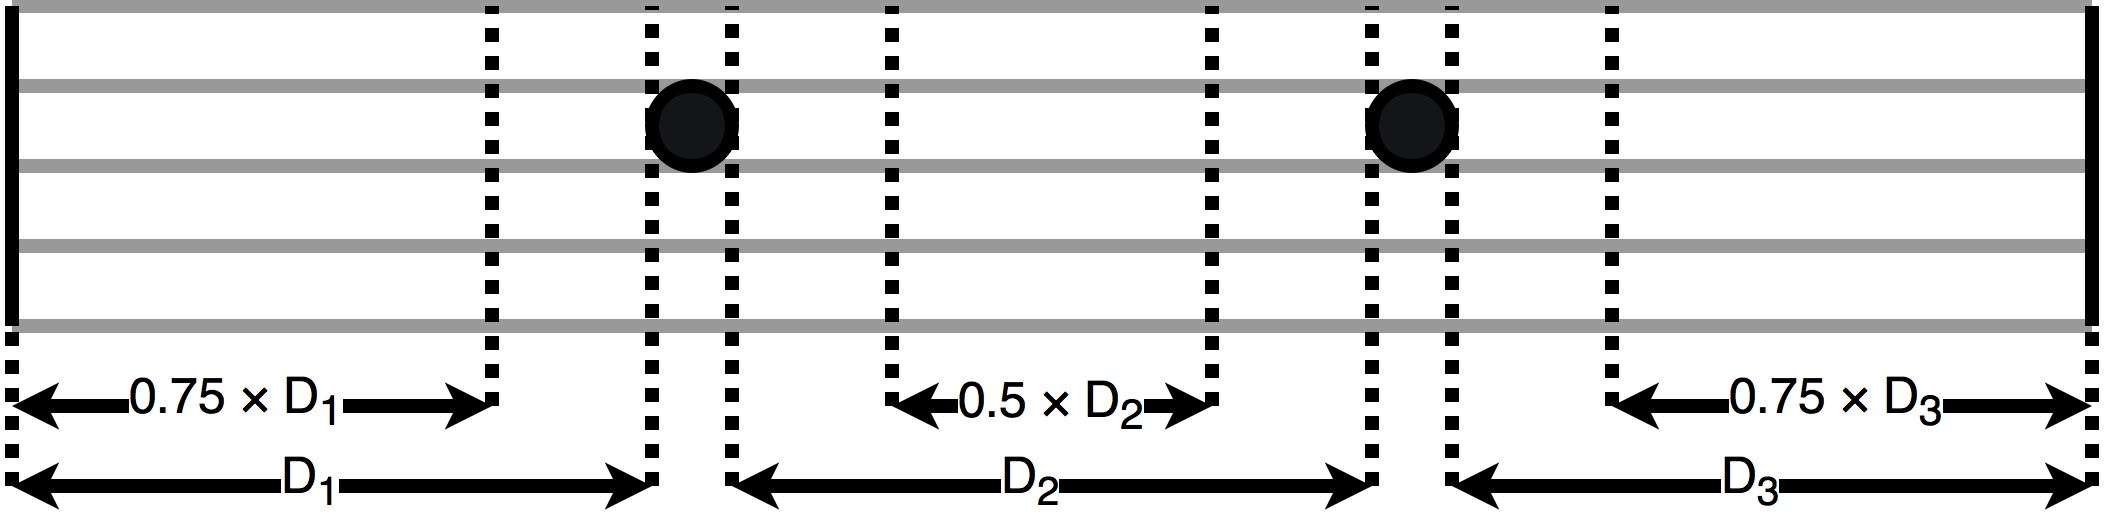
\includegraphics[scale=0.2]{imgs/hori-cutoff.png}
    \end{center}
    \caption{Horizontal Cutoff Zones}
    \label{fig:hori-cutoff}
\end{figure}

Next, to determine the bar line that was clicked, the $ y $ coordinate is compared against all the lines in the bar to
find the nearest line. A similar ratio based system as used with the $ x $ coordinate is used to determine if the cursor
should be placed between two lines or directly on a line. If the $ y $ coordinate is within the \textit{Space Zone} as
seen in Figure \ref{fig:vert-cutoff} then the cursor will be placed in the space between the two lines, but if the $ y $
coordinate is within the \textit{Line Zone} as seen in Figure \ref{fig:vert-cutoff} then the cursor will be placed on
the line within the zone. The line zones have to extend partially into the spaces between the lines because a line
itself is not tall enough to allow it to be clicked easily. These zones are implicit for spaces and lines above and
below the visible lines in the bar.

\begin{figure}[H]
    \begin{center}
        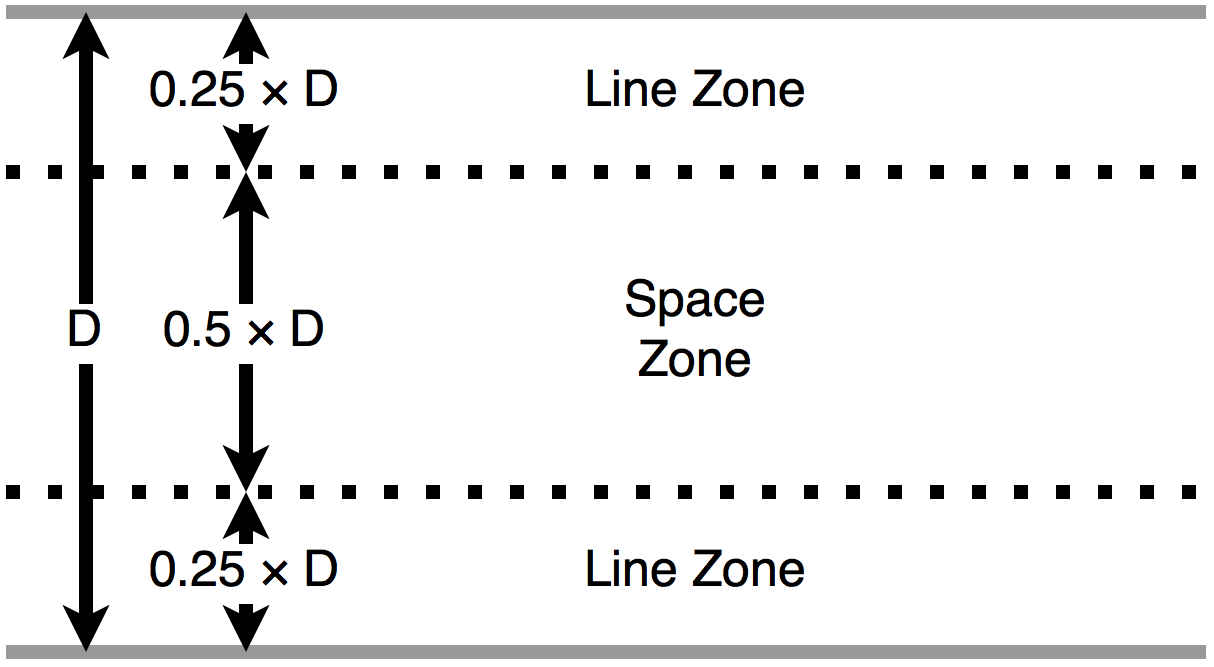
\includegraphics[scale=0.2]{imgs/vert-cutoff.png}
    \end{center}
    \caption{Vertical Cutoff Zones}
    \label{fig:vert-cutoff}
\end{figure}

With a cursor that stores the exact location of a click, modifying the score can be implemented, starting with adding
and removing measures. When a new measure is selected to be added, the new measure is created such that each bar in the
currently selected measure is duplicated except without all the notes and rests. Thus each bar in the new measure will
have the same time signature, key signature, and clef as the bar in the same staff as it. Then the new measure is added
after the currently selected measure. To delete a measure, as long as there is more than one measure, the currently
selected measure is removed from the list of measures. Due to reactivity in VueJS, when the list of measures is changed,
the entire layout is recalculated and redrawn automatically.

Continuing with the ability to expand the size of the music score, the next operations to implement is adding and
removing staffs, which includes adding and deleting groups. In this situation, the cursor is less important and is
purely used for user convenience. When the user selects to add a new staff, the user is prompted to select which group
(or instrument) the user wishes to add the staff to. The currently selected staff is used to find the appropriate group
and then that group is selected by default. The user can selected one of the existing groups, or they can create a new
group. If an existing group is selected a new bar is spliced into each measure at the end of the selected groups
section and the group's count is incremented. If the user selects to create a new group, a new bar is added to the end
of each measure and a group is added at the end of the list of groups with a count of one. Now that staffs can be added,
staffs need to be able to be deleted. To delete a staff, the currently selected staff is used to find the appropriate
group. As long as at least one staff exists, then each bar for the staff is removed from each measure and the
appropriate group's count is decreased by one. If the group's count reaches zero, then that group is also deleted. Due
to VueJS reactivity system, both adding and removing staffs will automatically redraw the music score.

Next the user needs to be able to change the time signature for each measure. To accomplish this, when the user selects
to edit the time signature the user is given ability to enter the upper and lower values for the time signature. The
default values in for the time signature inputs comes from the time signature of the currently selected measure. When
the user is finished the time signature of the currently selected measure is set to the new value. VueJS will detect the
change and the music score will automatically be redrawn.

The ability for the user to edit the clefs of bars is implemented next. When the user selects to edit the clef, the
user is given every possible clef as an option and the default selected clef is the clef of the currently selected bar.
After selecting the new clef, the clef of the currently selected bar is updated. The change will automatically be
detected by VueJS, and the music score will be redrawn.

Allowing the user to change the key signature of a bar is implemented similar to editing clefs. Thus, when a user
selects to edit the key signature, the user is given every possible key signature as an option and the default selected
key signature is the key signature of the currently selected bar. After selecting the new key signature, the key
signature of the currently selected bar is updated. As mentioned prior, VueJS will automatically detect the change and
the music score will be redrawn.

All that remains for user interaction is to allow notes and rests to be added and removed. How the user selects the
duration and whether or not the tick is a rest will be covered later, so assume the user has already selected the
settings for the note they wish to add. To add a note or a rest, the current cursor location is used to determine if a
new tick needs to be created, or if the duration of an existing tick needs to be updated. If a new tick needs to be
created it is spliced into the list of ticks at the cursor's location. If the user has selected a rest, then the tick
is cleared of all notes, otherwise the cursor's line and the clef of bar is used to lookup the correct note and the note
is added in the correct order. VexFlow expects notes to be ordered from highest to lowest. To delete a note, the
cursor's line is used to create the correct note for the line and the note is used to attempt to delete an equal note
from the selected tick. If it fails to delete the note, then the cursor isn't on a specific note, so the entire tick is
deleted. If the tick is a rest or deleting the note removes all notes in the tick, then the entire tick is also deleted.
VueJS will pick up any new or deleted ticks and notes and the music score will automatically be redrawn.

\section{Database Design}

MongoDB is the chosen database because it is a document database and with the JSON based data model for music scores it
allows the music score to be easily stored in a structure as close to the data model as possible. The detailed structure
of the MongoDB database can be seen in Appendix B. Before music scores can be persisted, an owner needs to be able to be
assigned to each music score. Thus before music scores can be saved, users need to exist to be assigned as owners.
Therefore a \lstinline{users} collection is required to get an ID for a user. The value of the \lstinline{_id} field for
a user that creates a music score is set as the value for the \lstinline{owner} field in the \lstinline{musicScores}
collection. A matching \lstinline{owner} field is added in the \lstinline{measures} collection. The value of the
\lstinline{_id} field for a music score is set as the value for the \lstinline{score} field in the \lstinline{measures}
collection to identify which measures belong to which music score.

The structure of the database needs to accomplish two main goals. First, as little measures as possible are to be loaded
from the database in order to perform the necessary music score changes. These measures will be modified by the server
and then published back to the database to be persisted. Ideally, only the measures that are actually modified should be
loaded from the database. Secondly, due to the concurrent nature of web applications, and the highly structured
nature of the music scores, each music score update needs to be atomically performed and any concurrent modifications
need to be detected and prevented. These two goals aim to make the updates to the music score efficient and aim to
prevent placing the music scores into invalid states.

To detect and prevent concurrent modifications, each music score has a \lstinline{rev} field, which is generated ID,
that keeps track of the current revision of the music score. When an update attempt is performed, the expected revision
is passed with the update operation; for the update to succeed, the current revision of the music score must match the
expected revision of the music score. Each measure in a music score has a matching \lstinline{rev} field (the reason the
field is a list is explained later), so for a measure to belong to the current music score one of its revisions
must equal the revision in the music score document.

To make each update atomic, the structure of the data is highly impacted by two implementation decisions in MongoDB.
Measures must be in their own collections, and cannot be an array in the music score, because Mongo does not allow
multiple elements in an array to be updated at the same time, unless the elements' indices are explicitly mentioned, and
an item cannot be removed from an array using the items index. As an example, in order to delete a measure, the ID of
the measure to delete and the index of both the next and previous measures would need to be known to perform the update
in a single operation. Since an index is unique for each measure and an ID is unique for each measure, practically
speaking, multiple IDs would need to be tracked for each measure, except in the case of the index the value would change
for every following measure if a measure before gets deleted. So not only would each measure have a stable ID, each
measure would have an unstable ID as well. This is becomes both time consuming in terms of always updating index values
as necessary and complex in keeping both IDs in sync. Thus measures are moved into their own collection with an ID and
without an index value; the IDs are not set as the \lstinline{_id} field because it is the \lstinline{id},
\lstinline{rev} combinations that will be unique, not the \lstinline{id} alone.

Now that each measure is its own document, a different implementation decision in MongoDB needs to be accounted for. In
MongoDB only writes to the same document are atomic, even for a single update statement. For example, assume there is a 
collection with multiple documents, all with the field \lstinline{foo = "bar"}, and an update attempts to set the
\lstinline{foo} field in all documents in the collection to the value \lstinline{"diff"}. During the update process, if
another operation attempts to read all the documents from the collection, it is possible for the read to get some 
documents with \lstinline{foo = "bar"} and some documents with \lstinline{foo = "diff"}. Due to the this behavior, there
needs to be a way to update all measures for a single music score in such a way that if a read operation occurs during
the update process, the read will always return a valid version of the music score.

To allow changes to be made to measures while keeping read results valid, each measure document is treated as immutable,
except for the \lstinline{rev} field. To allow untouched measures to not need to be replaced, the \lstinline{rev} field
is a list of valid revisions. This allows new measures to be written while the old measures exist, and measures
that don't change remain untouched; thus, the first goal of the database design can be achieved and unmodified measures
do not need to be replaced. The first operation during an update, is the generation of a new revision. Revisions need to
generated as opposed to incremented because multiple updates could be attempted at the same time, so these updates all
need a unique revision number. Then the updated measures are created with the new revision value, and a list of all new
IDs are kept track of; the IDs of the measures to delete are added to these IDs because excluding the actual creation of
the updated measures, the deletion process is the same as the cleanup process for old measures. Then all measures that
were not updated and are not to be deleted have the new revision added to their list of revisions. At this point all the
measures for the new revision exist in a valid state. Next the master revision in the music score is updated to the new
revision value; if a concurrent update occurred, then this update will fail and the initial setup of the measures can
easily be undone. With the master update complete, the music score is officially updated. To ensure the database does
not grow too fast, all the outdated measures must now be cleaned up; this includes deleting all the measures with the
old revision and whose ID is in the list of IDs created earlier and then removing all the remaining old revisions from
the other measures' revision lists.

Unfortunately, valid concurrent reads are not perfectly handled by the update process alone. In order to do a valid read
of the music score with its measures, the music score has to be read first to obtain the current revision. The revision
is then used to read all of the measures for the music score with a matching revision. Immediately after the first read
another concurrent operation could change the current revision and start cleaning up old measures before the first
operation starts reading the matching measures. Because of this edge case, after reading all the measures, a read
operation needs to read the revision from the music score document again to ensure it hasn't changed. If it has changed
the read operation needs to re-retrieve the measures with the new revision and perform the revision check again.

\section{Conclusion}

\subsection{Results}

\subsection{Future}

\newpage

\section{Appendices}

\subsection{Appendix A -- Data Model}

\begin{lstlisting}[language=json, caption=Note]
{
    "letter" : <String>,
    "octave" : <Number>,
    "accidental" : <String>
}
\end{lstlisting}

\begin{lstlisting}[language=json, caption=Tick]
{
    "duration" : <Number>,
    "notes" : [ <Note> ]
}
\end{lstlisting}

\begin{lstlisting}[language=json, caption=Bar]
{
    "clef" : <String>,
    "keySig" : <String>,
    "ticks" : [ <Tick> ]
}
\end{lstlisting}

\begin{lstlisting}[language=json, caption=TimeSignature]
{
    "upper" : <Number>,
    "lower" : <Number>
}
\end{lstlisting}

\begin{lstlisting}[language=json, caption=Measure]
{
    "timeSig" : <TimeSignature>,
    "bars" : [ <Bar> ],
    "id" : <String>,
    "prev" : <Measure>,
    "next" : <Measure>
}
\end{lstlisting}

\begin{lstlisting}[language=json, caption=Group]
{
    "name" : <String>,
    "abbr" : <String>,
    "count" : <Number>
}
\end{lstlisting}

\begin{lstlisting}[language=json, caption=MusicScore]
{
    "id" : <String>,
    "title" : <String>,
    "measures" : [ <Measure> ],
    "groups" : [ <Group> ],
    "rev" : <String>
}
\end{lstlisting}

\subsection{Appendix B -- MongoDB Collections}

\begin{lstlisting}[language=json, caption=users]
{
    "_id" : <ObjectId>,
    "username" : <String>,
    "password" : <String>
}
\end{lstlisting}

\begin{lstlisting}[language=json, caption=musicScores]
{
    "_id" : <ObjectId>,
    "owner" : <ObjectId>,
    "title" : <String>,
    "groups" : [
        {
            "name" : <String>,
            "abbr" : <String>,
            "count" : <Number>
        }
    ],
    "rev" : <ObjectId>
}
\end{lstlisting}

\begin{lstlisting}[language=json, caption=measures]
{
    "_id" : <ObjectId>,
    "owner" : <ObjectId>,
    "score" : <ObjectId>,
    "id" : <String>,
    "rev" : [
        <ObjectId>
    ],
    "timeSig" : {
        "upper" : <Number>,
        "lower" : <Number>
    },
    "bars" : [
        {
            "clef" : <String>,
            "keySig" : <String>,
            "ticks" : [
                {
                    "duration" : <Number>,
                    "notes" : [
                        {
                            "letter" : <String>,
                            "octave" : <Number>,
                            "accidental" : <String>
                        }
                    ]
                }
            ]
        }
    ],
    "prev" : <String> or null,
    "next" : <String> or null
}
\end{lstlisting}


\end{document}
